\documentclass[a4paper, oneside, final]{article}
\usepackage[T1]{fontenc}
\usepackage[utf8]{inputenc}
\usepackage[british]{babel}
\usepackage{amsmath}
\usepackage{amsthm}
\usepackage{verbatim}
\usepackage{listings}

\renewcommand{\britishhyphenmins}{22} 

\let\fref\undefined
\let\Fref\undefined

\usepackage{graphicx}
\usepackage{amssymb}

\setcounter{secnumdepth}{1} % Sæt overskriftsnummereringsdybde. Disable = -1.
\setlength{\parskip}{0.25in}

\pagestyle{plain}

\title{Topics in Programming Languages}

\begin{document}

\maketitle

\section{Eden}

\section{Par Monad}

The Par Monad was originally described in the paper ``A monad for deterministic parallelism''\cite{parmonad}. As the name suggests it is a monad for specifying pure parallel computations. It is especially well suited for dataflow networks. The purpose of this section is to make the reader comfortable with the Par Monad such that the next section will be understandable.

Given a computation in the Par Monad you can execute it concurrently with the current computation using the \texttt{fork} function. Computations in the \texttt{Par} monad can be extracted using the \texttt{runPar} function. \newline

\begin{lstlisting}[language=Haskell, frame=tb, basicstyle=\footnotesize]
fork :: Par () -> Par ()
runPar :: Par a -> a
\end{lstlisting}

The astute reader may notice that \texttt{fork} and \texttt{runPar} aren't very useful by themselves as you would never be able to read the values produced by the parallel computations. A way to communicate results from the child to the parent process is necessary; for this the Par monad uses a communication abstraction they call IVars. \texttt{IVar}'s also act as the entry point to the Par Monad. \newline

\begin{lstlisting}[language=Haskell, frame=tb, basicstyle=\footnotesize]
data IVar a 

new :: Par (IVar a)
get :: IVar a -> Par a
put :: NFData a => IVar a -> a -> Par ()
\end{lstlisting}

The \texttt{new} function creates a new IVar, \texttt{get} reads the value stored in the IVar and \texttt{put} writes a value to the IVar. If you invoke \texttt{get} on an empty \texttt{IVar} it will block until a value is stored in the \texttt{IVar}. Readers familiar with concurrent programming in Haskell may notice That this approach is very similar to the use of \texttt{MVar} with the main difference that IVars are write-once where \texttt{MVar}'s can be written multiple times.

These five functions are that is needed to write parallel programs using the Par Monad. The following listing shows a small example program taken from \texttt{Control.Monad.Par} on hackage\footnote{http://hackage.haskell.org/packages/archive/monad-par/0.1.0.1/doc/html/Control-Monad-Par.html} \newline

\begin{lstlisting}[language=Haskell, frame=tb, basicstyle=\footnotesize, numbers=left, numberstyle=\tiny]
runPar $ do
   [a,b,c,d] <- sequence [new,new,new,new]
   fork $ do x <- get a; put b (x+1)
   fork $ do x <- get a; put c (x+2)
   fork $ do x <- get b
             y <- get c 
             put d (x+y)
   fork $ do put a (3 :: Int)
   get d
\end{lstlisting}

On line 1 four \texttt{IVar}'s are created. Lines 2-8 creates tasks that read and write to different IVars in parallel. Line 9 reads the value stored in the IVar bound to d and as such this is the value returned by the entire program.The program is shown as a data-flow diagram below.

\begin{lstlisting}
                            a
                           / \  
                          b   c
                           \ /
                            d
\end{lstlisting}

This should be sufficient to understand the purpose and usage of the Par Monad.

\section{Implementing the Par Monad}

\section{Benchmarks}

We have performed some limited benchmarking of our implementation of
the Par backend, wherein we compare our performance to the default
implementation.  Tests were performed on
$\texttt{sci-0},\texttt{sci-1},\ldots,\texttt{sci-6}$, six computation
nodes available on the DIKU network, with each running a quad-core
2.40GHz Intel Xeon processor.  The \texttt{sci} systems are
virtualised servers, resulting in unknown network topography and
system load, which has resulted in some unpredictable variation in
performance, and while we re-ran some benchmarks multiple times to
obtain sensible results, there are still some inexplicable artifacts
left.  The benchmarks are thus not a very precise indication of the
ultimate performance potential of the EDI-based Par monad, but rather
a basic demonstration of the viability of the approach.  A serious
exploration of the implementation should involve benchmarks on
dedicated cluster computing systems.  Finally, note that it is not
possible to run the default Par monad implementation in a distributed
setting, hence it does not benefit from access to more than the four
CPUs available on a single machine.  The benchmark programs have been
taken from the \texttt{monad-par} package and were unmodified.
Specific parameters have been tuned to exhibit relatively long
runtimes and sensible chunking of parallel work, so the results should
not be dominated by startup overhead, or exhibit non-realistic
workloads.

Figure \ref{fig:blackscholes} shows results from an implementation of
the Black-Scholes equation, executed with parameters corresponding to
$20,000,000$ options divided into $1000$ blocks.  We observe
almost-linear scaling, but also significant overhead.  As the core of
the benchmark program is a naïve parallel map across a list of twenty
thousand elements (one process per element), this is not particularly
surprising, given that EDI threads are somewhat heavy compared to
lightweight GHC threads.

A probably best-case situation for our monad is shown in Figure
\ref{fig:parfib}.  The Parfib program computes a Fibonacci number
using the recursive formula $fib(n) = fib(n-1) + fib(n-2)$; running
the recursive calls in parallel, except when $n$ is less than a given
threshold.  In the benchmark, we compute $fib(50)$, with $n=30$ as the
threshold for switching to sequential computation, resulting in a
manageable (although still large) number of processes, each doing a
relatively work-intensive task (computing $fib(30)$).  As a
consequence, since the runtime is dominated by the actual work, the
increased overhead of EDI process creation and communication is not
very noticable, and we scale essentially linearly (except for a hiccup
at the very end, most likely due to virtualisation artifacts).

\begin{figure}
\caption{Black-Scholes}
\label{fig:blackscholes}
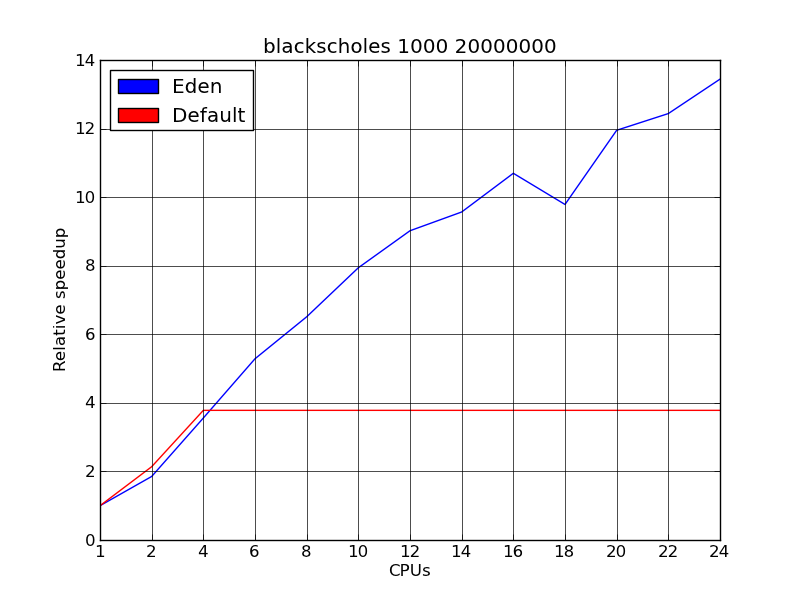
\includegraphics[width=7cm]{blackscholes-speedup.png}
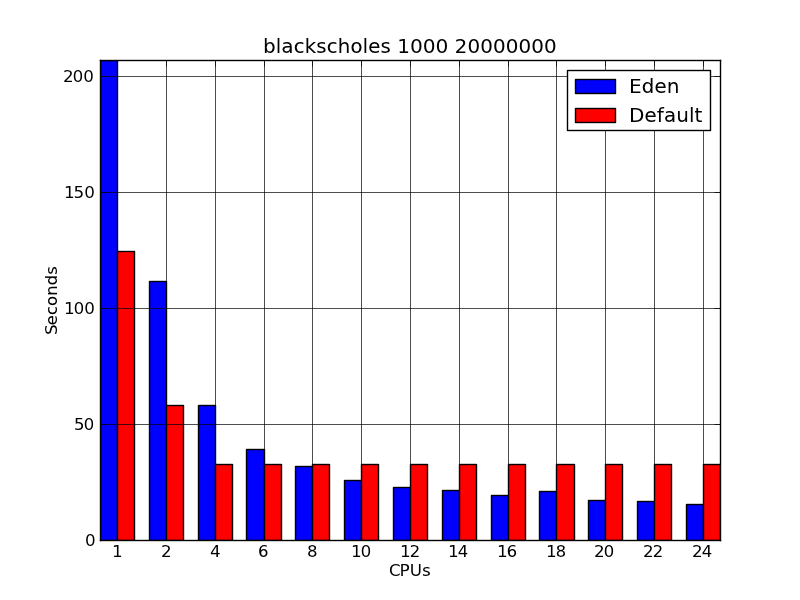
\includegraphics[width=7cm]{blackscholes-runtimes.png}
\end{figure}


\begin{figure}
\caption{Parallel computation of Fibonacci number}
\label{parfib}
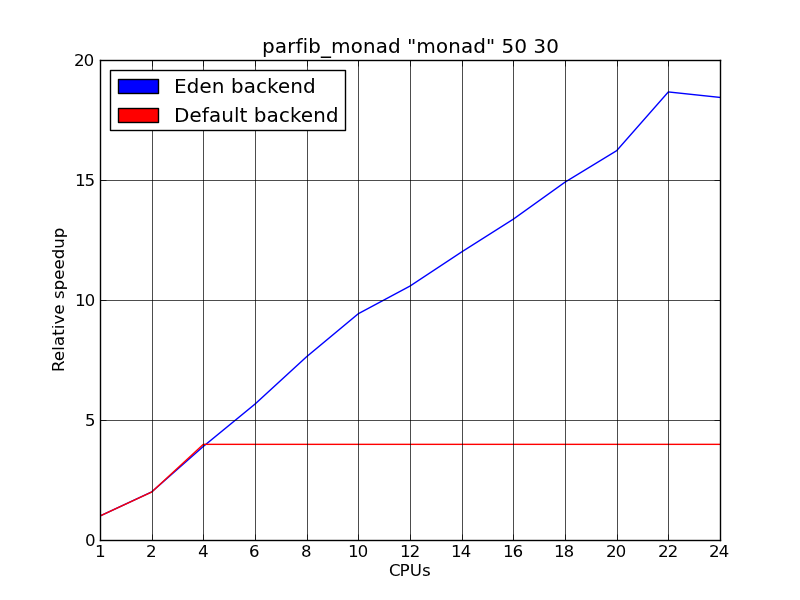
\includegraphics[width=7cm]{parfib_monad-speedup.png}
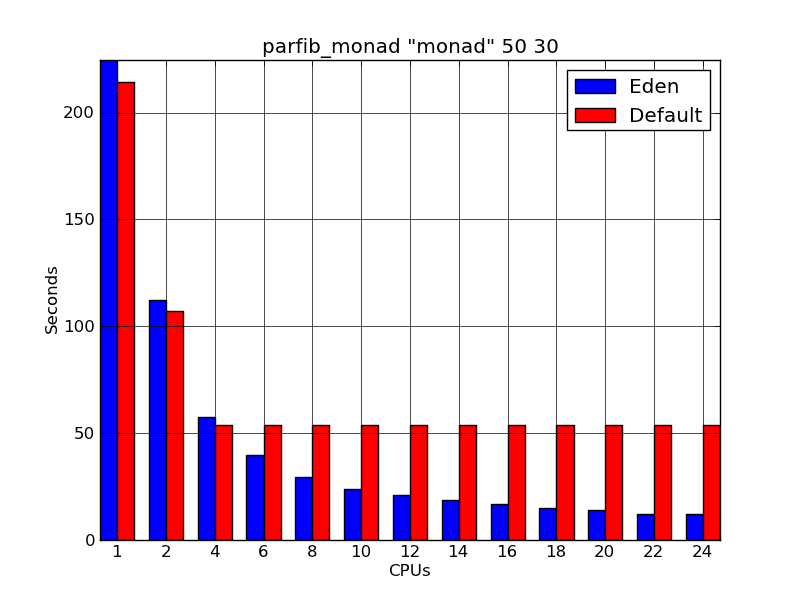
\includegraphics[width=7cm]{parfib_monad-runtimes.png}
\end{figure}

\section{Conclusion}

\bibliography{report}

\end{document}
